\documentclass[parskip]{scrartcl}
\usepackage[utf8]{inputenc}
\usepackage[ngerman,english]{babel}
\usepackage[round]{natbib}
\usepackage{graphicx,float,setspace,csquotes,amsmath,listings,url}
\usepackage[automark]{scrpage2}
\usepackage[usenames,dvipsnames]{color}
\usepackage[colorlinks=false, pdfborder={0 0 0}]{hyperref}
\lstset {
  language=java,
  basicstyle={\footnotesize\ttfamily},
  numbers=left,
  numbersep=-5pt,
  numberstyle=\tiny\color{Gray},
  aboveskip=11pt,
  belowskip=11pt,
  showstringspaces=false,
  columns=flexible,
  keywordstyle=\color{Fuchsia},
  identifierstyle=\color{Black},
  commentstyle=\color{ForestGreen},
  stringstyle=\color{blue},
  frame=single,
  breaklines=true,
  breakatwhitespace=true,
  tabsize=2,
  morekeywords={send,Response }% <-- adding custom keywords
}

\begin{document}
	\subject{Projektdokumentation im Modul Smartcard}
	\title{Patientendateninformationskarte im medizinischen Sektor}
	\author{Robert Kupferschmied B.Sc., Roy Meissner B.Sc.,\\Sebastian Krause B.Sc.}
	\date{\today}
	
	\maketitle
	
	\onehalfspacing
	\section{Anwendungsbeschreibung}
		Ziel der Anwendung ist es eine Smartcard mit Patientendaten zur Verfügung zu stellen, die im medizinischem Sektor Abläufe beschleunigt bzw. Automatisierung zulässt. Zu diesem Zweck stellt die Smartcard folgende Informationen bzgl. eines Patienten bereit:
		
		\begin{itemize}
			\item eine Patienten-ID
			\item die Patientenblutgruppe
			\item eine Liste nicht verträglicher Medikamente
			\item eine List regelmäßig einzunehmender Medikamente, incl. Dosierungsinformationen
		\end{itemize}
		
		Die Patientendaten auf der Smartcard können von verschiedenen Rollen (Personen) ausgelesen werden, die jeweils verschiedene Rechte besitzen. Beispielsweise darf ein Pfleger nur die Liste regelmäßig einzunehmender Medikamente auslesen, der Hausarzt darf hingegen alle Daten auslesen.
		
		Um die Datenübertragung zwischen Lesegerät bzw. Offcard-Software und Smartcard abzusichern, wird die Kommunikation kryptographisch gesichert. Zu diesem Zweck wird per RSA ein DES-Schlüssel ausgetauscht, der im folgenden den gesamten Datenverkehr verschlüsselt.
				
		Als Anwendungsfälle könnten gelten:
	
		\begin{description}
			\item[Notarzt] Im Falle eines Unfalls muss der Notarzt schnell auf Informationen wie Blutgruppe, nicht verträgliche Medikamente und aktuell verschriebene Medikamente zugreifen können, auch wenn der Patient bewusstlos ist. 
			\item[Automatisierte Medikamentenausgabe] Über die Liste regelmäßig einzunehmender Me\-dikamente, inklusive Dosierungsinformationen, könnten dem Patienten an einem Automaten Medikamente aushändigt werden.
		\end{description}
		
		\subsection{Aufgabenverteilung}
		Das gesamte Projekt wurde innerhalb der vergebenen Aufgabenbereiche zunächst separat entwickelt und am Ende zusammengeführt. Die Verantwortlichkeiten sind dabei der folgenden Tabelle zu entnehmen, haben sich bei der Zusammenführung jedoch nochmals überschnitten.
		
				\begin{table}[H]
					\centering
					\begin{tabular}[c]{|l|l|}
						\hline Name & Aufgabenbereich \\ 
						\hline
						\hline Krause, Sebastian & Offcard-Anwendung \\ 
						\hline Kupferschmied, Robert & Verschlüsselung/Kryptografie \\ 
						\hline Meissner, Roy  & Oncard-Anwendung \\ 
						\hline 
					\end{tabular} 
				\end{table}
		
		Die gesamte Dokumentation, der Code und eine Änderungshistorie kann auf Github gefunden werden. Das zugehörige Repository ist unter \url{https://github.com/neonlzf/smartcard} zu finden.
		
	\section{OffCard}
		Dieser Abschnitt beschreibt die OffCard-Anwendung und geht auf die zugrunde liegende Architektur ein.
	
	\subsection{Beschreibung der Offcard-Anwendung}
			Abbildung \ref{fig:maingui} zeigt das Hauptfenster der Offcard-Anwendung. Über die Schaltflächen "Load" und "Save" werden die Daten von der SmartCard gelesen bzw. auf die SmartCard geschrieben. Über das im oberen linken Teil des Fensters befindliche Drop-Down-Menü kann der jeweilige Akteur gewählt werden. So hat beispielsweise der Hausarzt vollen Zugriff, während der Pfleger nur Daten lesen kann.
	
		\begin{figure}[H]
			\centering
			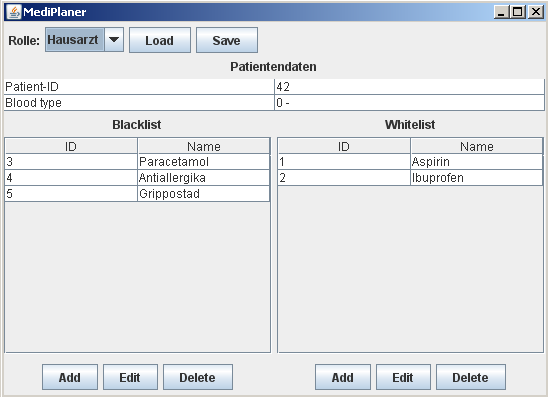
\includegraphics[width=.75\linewidth]{./maingui.png}
			\caption{Hauptfenster der Offcard-Anwendung}
			\label{fig:maingui}
		\end{figure}
		
		Im Bereich Patientendaten sind die Stammdaten des Patienten zu sehen. Dabei handelt es sich um seine ID, zb. die Krankenversicherungsnummer, und seine Blutgruppe. Durch die Speicherung einer eindeutigen ID, ist es möglich patientenbezogene Daten von Online-Diensten anzufordern und in die Anwendung einzubinden. Die Blutgruppe wird darüber hinaus als wichtige Information bereitgehalten.
		
		Darunter sind die Medikamenten-Whitelist und -Blacklist angeordnet. Diese können über Markierung und die Schaltflächen "Add", "Edit" und "Delete" bearbeitet werden.
		
		\begin{figure}[H]
			\centering
			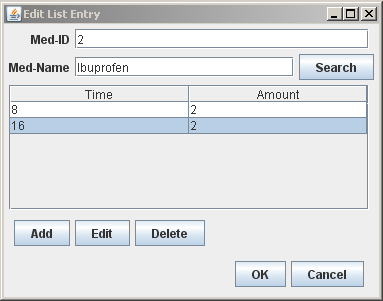
\includegraphics[width=.6\linewidth]{./mededitgui.png}
			\caption{Fenster für Medikamenteneditierung der Offcard-Anwendung}
			\label{fig:mededit}
		\end{figure}
		
		Die Abbildung \ref{fig:mededit} zeigt das Fenster zur Editierung eines Medikamentenlisteneintrages. Durch Eingabe eines Teilstrings im Feld "Med-Name" und anschließender Betätigung der "Search"-Schaltfläche wird aus den Medikamentenstammdaten der vollständige Name und die entsprechende Medikamenten-ID geladen. Diese Stammdaten werden in einer XML-Datei vorgehalten, welche zu Programmstart geladen wird.
		
		Des Weiteren enthält das Medikamenteneditierungsfenster eine Liste der vom Arzt vor\-ge\-schrie\-ben\-en Dosierungen, bestehend aus Uhrzeit in vollen Stunden und Einheiten. Diese kommt jedoch nur bei der Whitelist, der Liste einzunehmender Medikamente, zum Einsatz. 
		
		\begin{figure}[H]
			\centering
			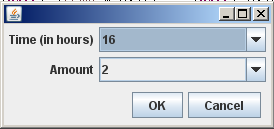
\includegraphics[width=.4\linewidth]{./dosageeditgui.png}
			\caption{Fenster zur Festlegung der Dosierung}
			\label{fig:dosageedit}
		\end{figure}
		
		Abbildung \ref{fig:dosageedit} stellt das Menü zur Bearbeitung eines Dosierungseintrages dar. Hier können Uhrzeit und Anzahl dieses Eintrages festgelegt werden.
		
		\subsection{Architektur}
		Im Bild \ref{fig:classdiagramm} ist das Klassendiagramm der Offcard-Anwendung zu sehen. Das Projekt ist dabei in die Pakete "card", "data" und "gui" unterteilt.
		
		\begin{figure}[H]
			\centering
			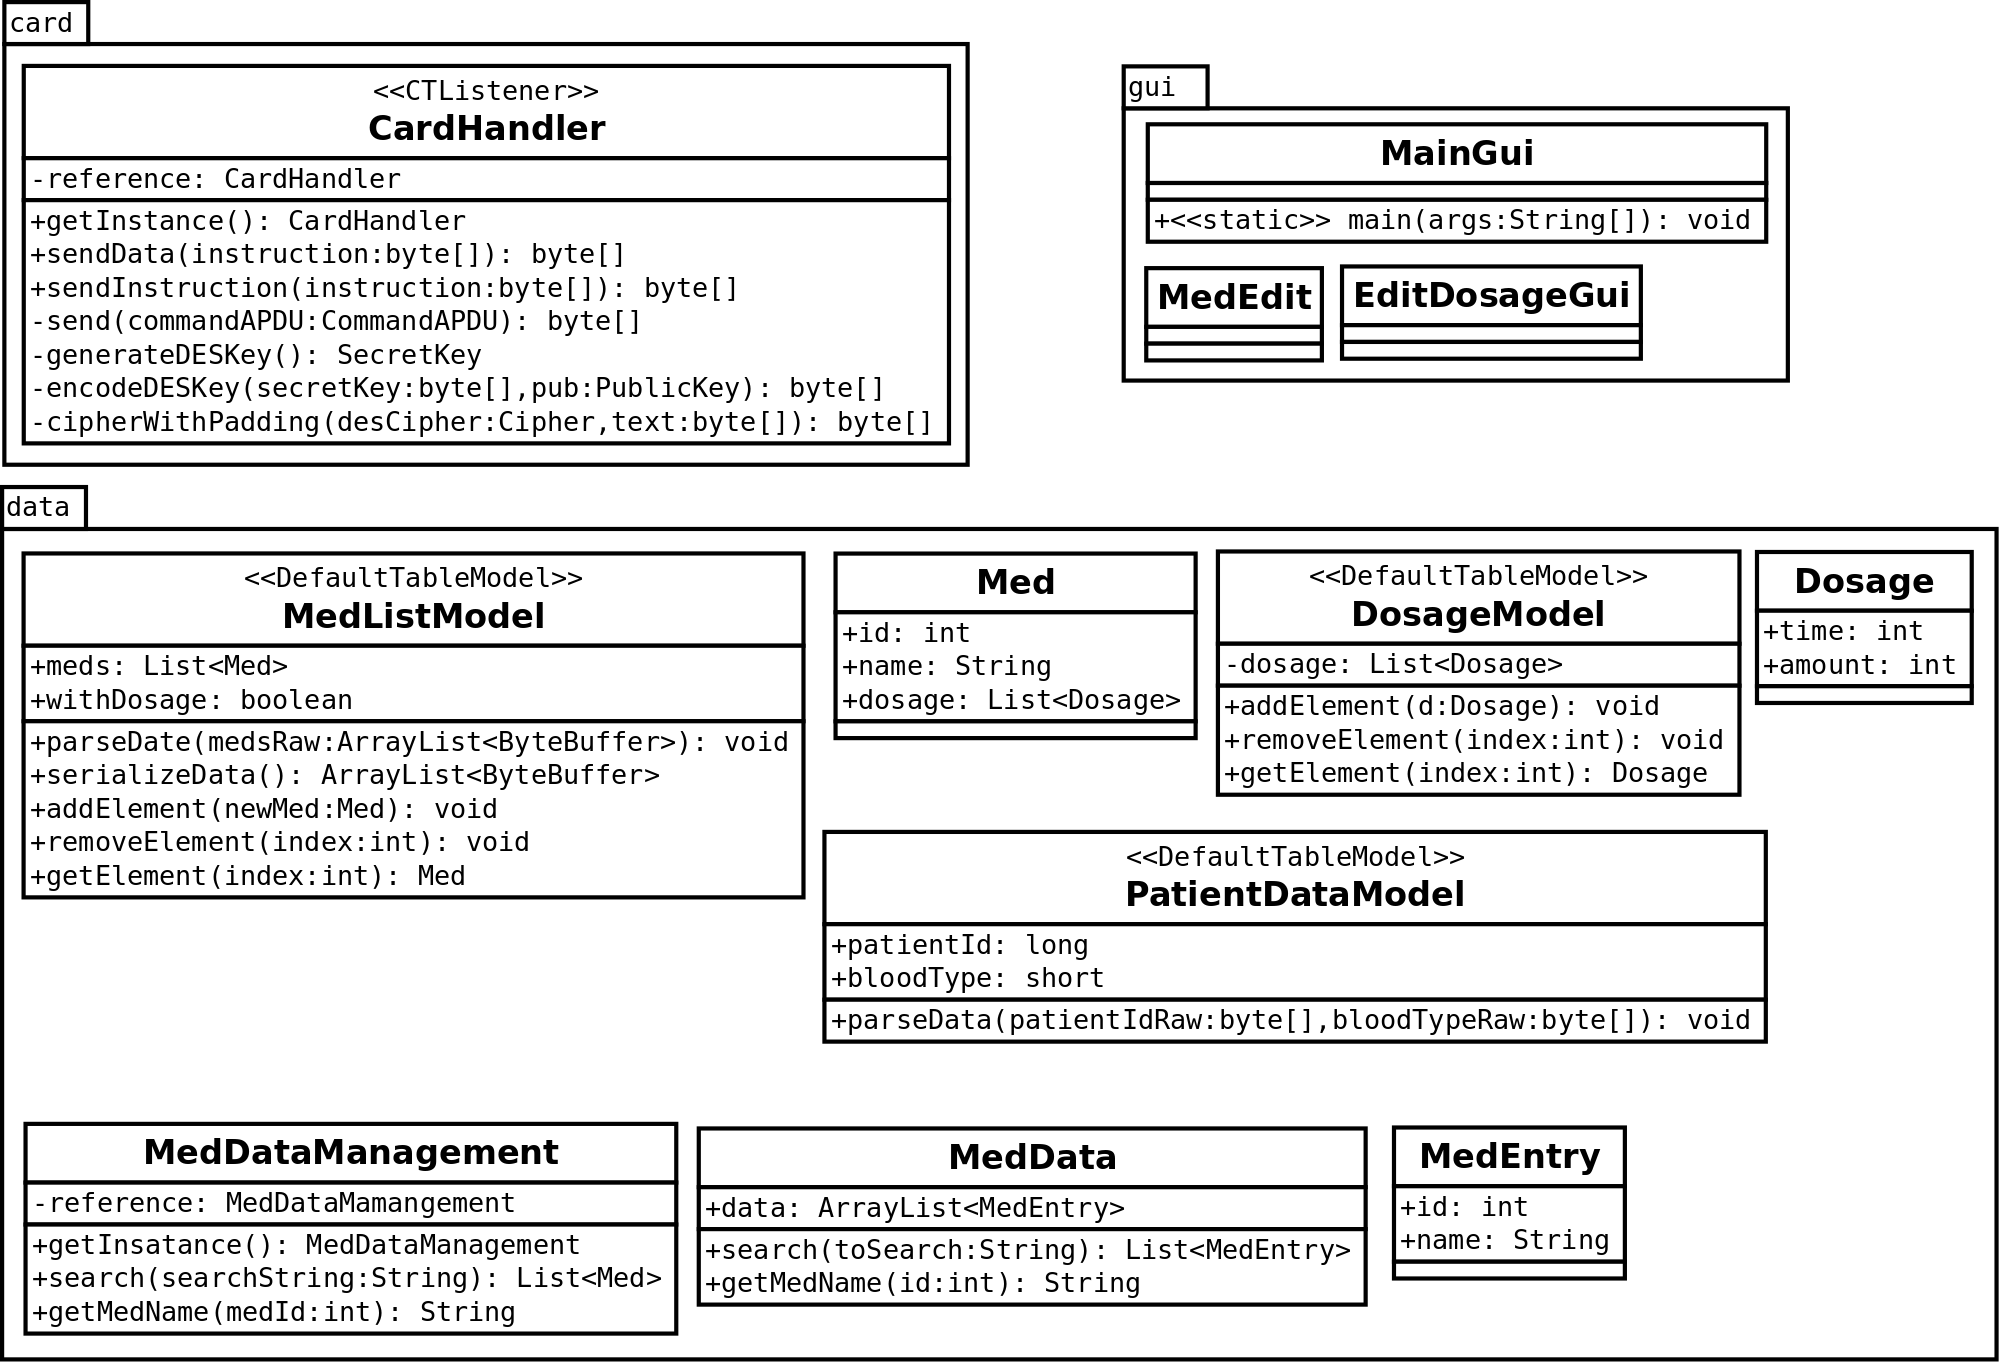
\includegraphics[width=\linewidth]{./klassendiagramm.png}
			\caption{Klassendiagramm der Offcard-Anwendung}
			\label{fig:classdiagramm}
		\end{figure}
		
		Im "card"-Paket befindet sich die Klasse "CardHandler". Diese kapselt den vollständigen Zugriff zur SmartCard und stellt darüber hinaus Methoden zur Verschlüsselung bereit. Realisiert ist die Klasse dabei als Singleton, um sicherzustellen, dass nur eine Instanz für die gesamte Anwendung instantiiert wird.
		
		Das Paket "gui" enthält die drei Klassen für die grafische Benutzeroberfläche. Darüber hinaus stellt "MainGui" die main-Methode zum Programmeinstieg bereit.
		
		Im Paket "data" liegen alle Klassen zur anwendungsseitigen Datenhaltung. Die Klasse "PatientDataModel" enthält die von der SmartCard gelesenen Stammdaten des Patienten. Die Klassen "MedListModel", "Med", "DosageModel" und "Dosage" kapseln die Daten der Medikamentenlisten. Die Model-Klassen erweitern "DefaultTableModel" um die Darstellung in einer Tabelle zu gewährleisten. Darüber hinaus enthalten "PatientDataModel" und "MedListModel" die Methoden "parseData()" und "serializeData()". Diese Klassen konvertieren die von der Karte gelesenen Byte-Arrays in von der Anwendung verarbeitbare Daten und zurück. 
		
		Zur Verwaltung der Medikamentenstammdaten dienen die Klassen "MedDataManagement", "MedData" und "MedEntry". Die eigentlichen Daten bilden dabei "MedData" und "MedEntry", wobei "MedDataManagement" zur Deserialisierung dieser aus einer XML-Datei dient. Dies wird über das JAXB-Framework realisiert.
	
	\section{OnCard}
		Die OnCard-Anwendung bietet eine vollständig definierte Schnittstelle in Form einer APDU-Beschreibung\footnote{in der Datei APDUs.txt zu finden} an. Über diese Schnittstelle kann mit den Daten, die auf der Smartcard gespeichert sind, interagiert werden.
		
		Die Patienten-ID wird zur Installation des Applets auf der Karte fest kodiert. Die ID ist eine Zahl vom Typ long, die auf der Smartcard in Form von 8 Bytes abgespeichert wird. Long wurde gewählt um jedem Menschen eine solche Karte aushändigen zu können, ohne das die IDs ausgehen. Die ID kann über die Schnittstelle nur abgerufen, jedoch nicht verändert werden.
		
		Ein beispielhafter Abruf der Patienten-ID sieht wie folgt aus:
		
		\begin{lstlisting}
			\send 00 08 00 00
			Response:
			00 00 00 00 00 00 00 01 90 00 //Patienten-ID + No-Error-Code
		\end{lstlisting}
		
		Die Blutgruppe des Patienten wird, wie die Patienten-ID, zur Installation des Applets festgelegt. Sie ist als ein Byte codiert und kann anhand einer Kodierungstabelle\footnote{diese ist in der Datei APDUs.txt zu finden} übersetzt werden. Wie die Patienten-ID ist auch die Blutgruppe nicht manipulierbar.
		
		Ein beispielhafter Abruf der Patienten Blutgruppe sieht wie folgt aus:
		
		\begin{lstlisting}
			\send 00 07 00 00
			Response:
			04 90 00 //Bloodtype + No-Error-Code
		\end{lstlisting}
		
		Auf der Smartcard wird eine Liste nicht verträglicher Medikamente gespeichert. Diese ist als eine List von jeweils 4 Byte IDs angelegt. Diese können in der OffCard-Anwendung in ein Int umgewandelt und über eine Kodierungstabelle dem entsprechenden Medikament zugeordnet werden. Die Smartcard bietet an, die Liste Elementweise auszulesen, neue Medikamente zur Liste hinzuzufügen, als auch die Liste zu verwerfen.
		
		Ein beispielhaftes Hinzufügen eines Medikaments zur Liste sieht wie folgt aus:
		
		\begin{lstlisting}
			\send 00 02 00 00 04 00 00 42 83 //Add Element with ID 00 00 42 83
			Response:
			Success: 90 00
			Failure: 6A 83
		\end{lstlisting}
		
		Ein beispielhafter Abruf eines Medikaments der Liste sieht wie folgt aus:
		
		\begin{lstlisting}
			\send 00 01 00 09 //Fetch Element 9
			Response:
			Success: 00 00 42 83 90 00 //Drug-ID + No-Error-Code
			Failure: 6A 83
		\end{lstlisting}
		
		Ein beispielhaftes Löschen der Liste sieht wie folgt aus:
			
		\begin{lstlisting}
			\send 00 03 00 00
			Response:
			90 00
		\end{lstlisting}
		
		Die Liste der regelmäßig einzunehmenden Medikamente ist gleich der Liste nicht verträg\-licher Medikamente aufgebaut, einzig die Eintragslänge entspricht im Gegensatz 28 Byte. Die ersten 4 Byte entsprechen der Medikamenten-ID, die folgenden 24 Byte den Einnahmezeiträumen sowie der Einnahmemenge. Diese Liste kann über die gleichen Methoden wie die Liste der nicht verträglichen Medikamente ausgelesen bzw. manipuliert werden.
		
		Intern werden die Listen über eine, eigens für diesen Zweck entwickelte, Datenstruktur organisiert. Diese bietet ein Ressourcenschonendes List-Interface für das kontrollierte Hinzufügen und Auslesen der Listenelemente, als auch ein verwerfen der gesamten Liste.
		
		Alle zwischen der OnCard- und der OffCard-Anwendung übertragenen Daten werden verschlüsselt. Zu diesem Zweck bietet der OnCard zwei Funktionen, um den Public RSA-Key Exponenten und Modulus exportieren zu können. Aus diesen kann sich die OffCard-Anwendung den Public-RSA-Key der SmartCard errechnen und mit diesem den DES-Key verschlüsseln. Dieser wird zur SmartCard übertragen und für die Lebenszeit der Session gespeichert. Mit diesem DES-Key wird wiederum jedwede Datenübertragung gesichert, egal ob ankommende Daten oder ausgehende Daten.
	\section{Kryptologie}
		In diesem Kapitel werden die kryptografischen Methoden des Projektes erklärt. Zum Verschlüsseln der Daten wird ein symmetrisches Verfahren verwendet. Symmetrische Verschlüsselungsverfahren sind sehr effizient und sicher. Leider werden bei symmet\-rischen Verfahren nur ein Schlüssel zum Ver- und Entschlüsseln verwendet. Deswegen ist der Schlüsselaustausch sehr schwierig. Asymmetrische Verfahren können dieses Problem lösen.
		\subsection{Asymmetrische Verschlüsselung - RSA}
			Zur asymmetrischen Verschlüsselung stehen auf den Smartcards prinzipiell zwei Algorithmen zur Verfügung. Zum einen der \enquote{elliptic Curve}-Algorithmus und der RSA\footnote{Rivest, Shamir und Adleman}-Algorithmus. Die Sicherheit des RSA-Algorithmus beruht auf dem Problem der Prim\-zahl\-zerlegung. Das Problem der Primzahlzerlegung ist ein schwieriges Problem, da kein effizienter Algorithmus bekannt ist der das Problem lösen könnte. Weiterhin ist RSA der bekannteste und am weitesten verbreitete Algorithmus zur asymmetrischen Verschlüsselung. Um zu möglichst vielen Systemen kompatibel zu sein, wird der RSA-Algorithmus in diesem Projekt verwendet.
			
			Bei asymmetrischen Verschlüsselungsverfahren werden Schlüsselpaare für die Verschlüs\-selung benutzt. Diese Schlüsselpaare bestehen aus einem Public-Key und einem Private-Key. Der Public-Key kann publiziert werden. Den Private-Key muss man geheim halten.
		
			Die Schlüssel setzen sich aus einem Exponenten und einem Modulus zusammen. Der Modulus ist eine sehr große Zahl, bei RSA-1024 eine Zahl im Bereich von $ 2^{1024} $ und setzt sich aus zwei Primzahlen zusammen. Der Modulus ist im Public- und Private-Key gleich. Die Exponenten unterscheiden sich allerdings.
		
			Zur Ver- und Entschlüsselung werden folgende Funktionen benutzt:  
			 $$ G = K^{e}\mod{n} $$
			 $$ K = G^{d}\mod{n} $$
			 \begin{align*}
			  G & \text{ ... Geheimtext} & K & \text{ ... Klartext} \\
			  e & \text{ ... öffentlicher Exponent} & d & \text{ ... geheimer Exponent} \\
			  n & \text{ ... Modulus} & &
			 \end{align*}
			 
			Die Schlüssel werden in der Datei \enquote{irgendwas.java} erzeugt. Hier sind diese Zeilen wichtig:
			\label{RSAKeyPair}
			\begin{lstlisting}
				Cipher rsaCipher = Cipher.getInstance(Cipher.ALG_RSA_PKCS1,false);
				KeyPair keyPair = new KeyPair(KeyPair.ALG_RSA_CRT, (short)1024);
				keyPair.genKeyPair();
				RSAPrivateCrtKey rsa_privateKey = (RSAPrivateCrtKey) keyPair.getPrivate();
				RSAPublicKey rsa_publicKey = (RSAPublicKey) keyPair.getPublic();
			\end{lstlisting}
			Die JCOP Shell hat beim Erstellen der Schlüssel leider ein paar Fehler. Hier kann beim Erzeugen des öffentlichen Schlüssels kein echter öffentlicher Exponent erzeugt werden, stattdessen wird nur eine konstante binäre 17 zurückgegeben.
		
			Auf einer echten Karte dürfte dieser Fehler nicht auftreten.
		
			Die Verschlüsselung mit asymmetrischen Verfahren ist nicht so effizient, wie die Verschlüsselung mit symmetrischen Verfahren. Deswegen ist es sinnvoll die symmetrische und asymmetrische Verfahren zu kombinieren um die Vorteile aufzuwiegen. Asymmetrische Verfahren werden dazu verwendet um den Schlüssel der symmetrischen Verfahren auszutauschen.
	
		\subsection{Symetrische Verschlüsselung - DES, AES}
			Für die symmetrische Verschlüsselung ist nur ein Schlüssel für die Ver- und Entschlüs\-selung notwendig. Dieser wird von dem Off-Card Programm erzeugt und via RSA-Verschlüs\-selung an die Karte gesendet. Als Verschlüsselungsalgorithmus wird DES benutzt. Dieser besitzt eine Schlüssellänge von 56-Bit. DES gilt nicht mehr als sicher da die Schlüssellänge zu kurz ist. Normalerweise nutzt man bei der modernen Verschlüsselung AES. Dieser gilt als mathematisch sicher und man kann ihn nur angreifen indem man alle möglichen Schlüssel durchprobiert. AES besitzt einen Schlüsselraum von 128 Bit und kann auf 256 Bit erweitert werden.
			
			AES wird nicht von der Simulationsumgebung JCOP unterstützt, deswegen muss man DES einsetzen. Im Betrieb mit einer echten Karte sollte man allerdings AES verwenden.
			
			Sowohl AES als auch DES verschlüsseln die Daten Blockweise. Deswegen gibt es verschiedene Modi beim Verschlüsseln. Hier kann man folgende Modi einstellen:
			
			\begin{lstlisting}
				Cipher.getInstance(Cipher.ALG_DES_ECB_NOPAD,false);
				Cipher.getInstance(Cipher.ALG_DES_ECB_PKCS5,false);
			\end{lstlisting}
			
			Das Cipher-Objekt spricht den Kryptologie-Prozessor der Smartcard an. Der Algorithmus ist DES. ECB steht für Electronic Code Book, dies ist besonderer Sicherheitsmodus damit ähnliche Daten nicht erkannt werden. NOPAD steht für No Padding, hier können nur Daten verschlüsselt werden deren Länge ein vielfaches der Blocklänge entspricht. Im Modus PKCS5 wird der Klartext um die fehlenden Bytes ergänzt.
				
	\section{OpenCard Framework - OCF}
		Das OpenCard Framework ist eine Smartcard Middleware. Hiermit kann man mit Smartcards kommunizieren. Das OpenCard Framework ist komplett in Java programmiert und damit Betriebssystemunabhängig.
		
		Um mit einer Smartcard kommunizieren zu können, muss man zunächst die Verbindung aufbauen. Dafür ist folgende Methoden ausführen:
		
		\begin{lstlisting}
			CardRequest cardRequest = new CardRequest(CardRequest.ANYCARD, null, PassThruCardService.class);
			cardRequest.setTimeout(1);
			card = SmartCard.waitForCard(cardRequest);
		\end{lstlisting}
		
		Nun kann man über die \enquote{card} Variable APDU's an die Smartcard senden. Hierfür muss man folgende Methoden senden:
		
		\begin{lstlisting}
			CommandAPDU commandAPDU = new CommandAPDU(instruction.length);
			commandAPDU.setLength(instruction.length);
			System.arraycopy(instruction, 0, commandAPDU.getBuffer(), 0, instruction.length);
			PassThruCardService passThru = (PassThruCardService) card.getCardService(PassThruCardService.class, true);
			ResponseAPDU responseAPDU1 = passThru.sendCommandAPDU(commandAPDU);
		\end{lstlisting}
		
		Zunächst wird eine APDU angelegt, danach kann man sie mit Bytes beschreiben. Über den Befehl \enquote{sendCommandAPDU} wird die APDU an die Smartcard gesendet und als Rückgabewert wird die empfangene APDU zurückgeben.
		
	\section{Schlüsselaustausch mit OCF}
		Die Abbildung \ref{fig:KeyExchange} visualisiert den Ablauf.
		
		\begin{figure}[H]
			\centering
			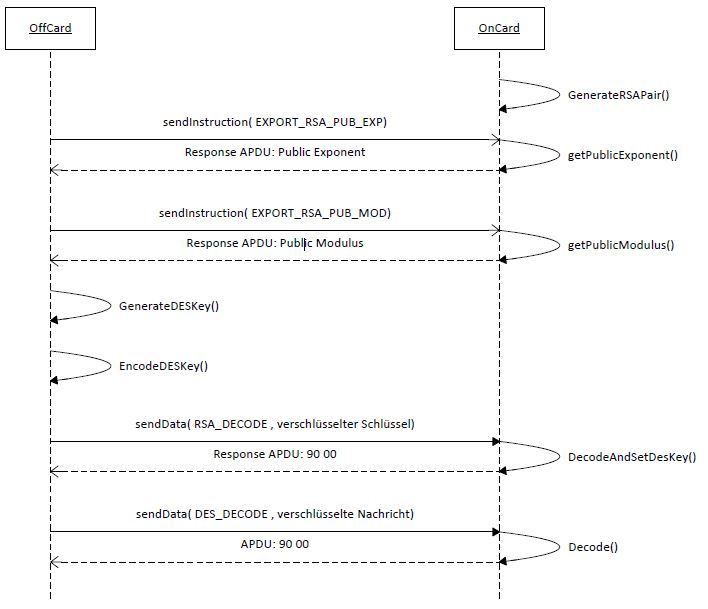
\includegraphics[width=\linewidth]{./KeyExchange}
			\caption{Schlüsselaustausch}
			\label{fig:KeyExchange}
		\end{figure}
		
		\begin{table}[H]
			\centering
			\begin{tabular}[c]{|l|l|}
				\hline Funktion & befindet sich in Datei \\ 
				\hline
				\hline sendInstruction( ) & CardHandler.java \\ 
				\hline sendData( ) & CardHandler.java \\ 
				\hline GenerateRSAPair()  & Patient.java \\ 
				\hline getPublicExponent() & Patient.java \\ 
				\hline getPublicModulus() & Patient.java \\ 
				\hline GenerateDESKey() & CardHandler.java \\ 
				\hline EncodeDESKey() & CardHandler.java \\
				\hline DecodeAndSetDesKey() & Patient.java \\
				\hline Decode() & Patient.java \\
				\hline 
			\end{tabular} 
		\end{table}
		
		\newpage
		Beim installieren der Smartcard-Applikation wird ein RSA Schlüsselpaar erzeugt. Dies geschieht über die in Kapitel \ref{RSAKeyPair}. Über die definierten Kommando APDU's \\\enquote{EXPORT\_RSA\_PUB\_EXP} und \enquote{EXPORT\_RSA\_PUB\_MOD} kann man sich den Pub\-lic-Key der Karte ausgeben lassen. Der Exponent und Modulus könne in Java durch die BigInteger-Klasse zu einem RSA-Key zusammengesetzt werden. Dann wird der DES-Key von der OffCard-Anwendung erzeugt. Diesen kann man nun mit RSA verschlüsseln und an die Karte senden. In der Karte wird der Schlüssl mit dem privaten RSA-Schlüssel entschlüsselt. Nun ist der DES-Schlüssel ausgetauscht und man kann effizient symmetrisch verschlüsseln. Um mit DES ver- und entschlüsseln zu können ist es wichtig die richtigen Modi einzustellen. Die virtuelle Karte von JCOP unterstützt nicht alle Modi. Wenn man den CBC\footnote{Cipher Block Chaining}-Modus einstellt entschlüsselt die virtuelle Karte nicht korrekt. Dies kann jedoch auch auf eine Inkompatibilität zwischen dem Ver- und Entschlüsselungsalgorithmus von Java und JavaCard hinweisen. Wenn man den Modus ECB\footnote{Eletronic Code Book} einstellt wird korrekt entschlüsselt. 
\end{document}